\documentclass[11pt,journal,compsoc]{IEEEtran}
% *** MISC UTILITY PACKAGES ***
%
%\usepackage{ifpdf}
% Heiko Oberdiek's ifpdf.sty is very useful if you need conditional
% compilation based on whether the output is pdf or dvi.
% usage:
% \ifpdf
%   % pdf code
% \else
%   % dvi code
% \fi
% The latest version of ifpdf.sty can be obtained from:
% http://www.ctan.org/tex-archive/macros/latex/contrib/oberdiek/
% Also, note that IEEEtran.cls V1.7 and later provides a builtin
% \ifCLASSINFOpdf conditional that works the same way.
% When switching from latex to pdflatex and vice-versa, the compiler may
% have to be run twice to clear warning/error messages.






% *** CITATION PACKAGES ***
%
\ifCLASSOPTIONcompsoc
  % IEEE Computer Society needs nocompress option
  % requires cite.sty v4.0 or later (November 2003)
  % \usepackage[nocompress]{cite}
\else
  % normal IEEE
  % \usepackage{cite}
\fi
% cite.sty was written by Donald Arseneau
% V1.6 and later of IEEEtran pre-defines the format of the cite.sty package
% \cite{} output to follow that of IEEE. Loading the cite package will
% result in citation numbers being automatically sorted and properly
% "compressed/ranged". e.g., [1], [9], [2], [7], [5], [6] without using
% cite.sty will become [1], [2], [5]--[7], [9] using cite.sty. cite.sty's
% \cite will automatically add leading space, if needed. Use cite.sty's
% noadjust option (cite.sty V3.8 and later) if you want to turn this off.
% cite.sty is already installed on most LaTeX systems. Be sure and use
% version 4.0 (2003-05-27) and later if using hyperref.sty. cite.sty does
% not currently provide for hyperlinked citations.
% The latest version can be obtained at:
% http://www.ctan.org/tex-archive/macros/latex/contrib/cite/
% The documentation is contained in the cite.sty file itself.
%
% Note that some packages require special options to format as the Computer
% Society requires. In particular, Computer Society  papers do not use
% compressed citation ranges as is done in typical IEEE papers
% (e.g., [1]-[4]). Instead, they list every citation separately in order
% (e.g., [1], [2], [3], [4]). To get the latter we need to load the cite
% package with the nocompress option which is supported by cite.sty v4.0
% and later. Note also the use of a CLASSOPTION conditional provided by
% IEEEtran.cls V1.7 and later.





% *** GRAPHICS RELATED PACKAGES ***
%
\ifCLASSINFOpdf
  % \usepackage[pdftex]{graphicx}
  % declare the path(s) where your graphic files are
  % \graphicspath{{../pdf/}{../jpeg/}}
  % and their extensions so you won't have to specify these with
  % every instance of \includegraphics
  % \DeclareGraphicsExtensions{.pdf,.jpeg,.png}
\else
  % or other class option (dvipsone, dvipdf, if not using dvips). graphicx
  % will default to the driver specified in the system graphics.cfg if no
  % driver is specified.
  % \usepackage[dvips]{graphicx}
  % declare the path(s) where your graphic files are
  % \graphicspath{{../eps/}}
  % and their extensions so you won't have to specify these with
  % every instance of \includegraphics
  % \DeclareGraphicsExtensions{.eps}
\fi
% graphicx was written by David Carlisle and Sebastian Rahtz. It is
% required if you want graphics, photos, etc. graphicx.sty is already
% installed on most LaTeX systems. The latest version and documentation can
% be obtained at: 
% http://www.ctan.org/tex-archive/macros/latex/required/graphics/
% Another good source of documentation is "Using Imported Graphics in
% LaTeX2e" by Keith Reckdahl which can be found as epslatex.ps or
% epslatex.pdf at: http://www.ctan.org/tex-archive/info/
%
% latex, and pdflatex in dvi mode, support graphics in encapsulated
% postscript (.eps) format. pdflatex in pdf mode supports graphics
% in .pdf, .jpeg, .png and .mps (metapost) formats. Users should ensure
% that all non-photo figures use a vector format (.eps, .pdf, .mps) and
% not a bitmapped formats (.jpeg, .png). IEEE frowns on bitmapped formats
% which can result in "jaggedy"/blurry rendering of lines and letters as
% well as large increases in file sizes.
%

%\usepackage[cmex10]{amsmath}
\usepackage{algorithmic}
\usepackage{amsmath,amssymb,amsthm}
\usepackage{graphicx}
%\usepackage{array}
%\usepackage{mdwmath}
%\usepackage{mdwtab}
%\usepackage{eqparbox}
\usepackage[justification=centering]{caption}





% *** SUBFIGURE PACKAGES ***
%\ifCLASSOPTIONcompsoc
%\usepackage[tight,normalsize,sf,SF]{subfigure}
%\else
%\usepackage[tight,footnotesize]{subfigure}
%\fi
% subfigure.sty was written by Steven Douglas Cochran. This package makes it
% easy to put subfigures in your figures. e.g., "Figure 1a and 1b". For IEEE
% work, it is a good idea to load it with the tight package option to reduce
% the amount of white space around the subfigures. Computer Society papers
% use a larger font and \sffamily font for their captions, hence the
% additional options needed under compsoc mode. subfigure.sty is already
% installed on most LaTeX systems. The latest version and documentation can
% be obtained at:
% http://www.ctan.org/tex-archive/obsolete/macros/latex/contrib/subfigure/
% subfigure.sty has been superceeded by subfig.sty.


%\ifCLASSOPTIONcompsoc
%  \usepackage[caption=false]{caption}
%  \usepackage[font=normalsize,labelfont=sf,textfont=sf]{subfig}
%\else
%  \usepackage[caption=false]{caption}
%  \usepackage[font=footnotesize]{subfig}
%\fi
% subfig.sty, also written by Steven Douglas Cochran, is the modern
% replacement for subfigure.sty. However, subfig.sty requires and
% automatically loads Axel Sommerfeldt's caption.sty which will override
% IEEEtran.cls handling of captions and this will result in nonIEEE style
% figure/table captions. To prevent this problem, be sure and preload
% caption.sty with its "caption=false" package option. This is will preserve
% IEEEtran.cls handing of captions. Version 1.3 (2005/06/28) and later 
% (recommended due to many improvements over 1.2) of subfig.sty supports
% the caption=false option directly:
%\ifCLASSOPTIONcompsoc
%  \usepackage[caption=false,font=normalsize,labelfont=sf,textfont=sf]{subfig}
%\else
%  \usepackage[caption=false,font=footnotesize]{subfig}
%\fi
%
% The latest version and documentation can be obtained at:
% http://www.ctan.org/tex-archive/macros/latex/contrib/subfig/
% The latest version and documentation of caption.sty can be obtained at:
% http://www.ctan.org/tex-archive/macros/latex/contrib/caption/




% *** FLOAT PACKAGES ***
%
%\usepackage{fixltx2e}
% fixltx2e, the successor to the earlier fix2col.sty, was written by
% Frank Mittelbach and David Carlisle. This package corrects a few problems
% in the LaTeX2e kernel, the most notable of which is that in current
% LaTeX2e releases, the ordering of single and double column floats is not
% guaranteed to be preserved. Thus, an unpatched LaTeX2e can allow a
% single column figure to be placed prior to an earlier double column
% figure. The latest version and documentation can be found at:
% http://www.ctan.org/tex-archive/macros/latex/base/



%\usepackage{stfloats}
% stfloats.sty was written by Sigitas Tolusis. This package gives LaTeX2e
% the ability to do double column floats at the bottom of the page as well
% as the top. (e.g., "\begin{figure*}[!b]" is not normally possible in
% LaTeX2e). It also provides a command:
%\fnbelowfloat
% to enable the placement of footnotes below bottom floats (the standard
% LaTeX2e kernel puts them above bottom floats). This is an invasive package
% which rewrites many portions of the LaTeX2e float routines. It may not work
% with other packages that modify the LaTeX2e float routines. The latest
% version and documentation can be obtained at:
% http://www.ctan.org/tex-archive/macros/latex/contrib/sttools/
% Documentation is contained in the stfloats.sty comments as well as in the
% presfull.pdf file. Do not use the stfloats baselinefloat ability as IEEE
% does not allow \baselineskip to stretch. Authors submitting work to the
% IEEE should note that IEEE rarely uses double column equations and
% that authors should try to avoid such use. Do not be tempted to use the
% cuted.sty or midfloat.sty packages (also by Sigitas Tolusis) as IEEE does
% not format its papers in such ways.




%\ifCLASSOPTIONcaptionsoff
%  \usepackage[nomarkers]{endfloat}
% \let\MYoriglatexcaption\caption
% \renewcommand{\caption}[2][\relax]{\MYoriglatexcaption[#2]{#2}}
%\fi
% endfloat.sty was written by James Darrell McCauley and Jeff Goldberg.
% This package may be useful when used in conjunction with IEEEtran.cls'
% captionsoff option. Some IEEE journals/societies require that submissions
% have lists of figures/tables at the end of the paper and that
% figures/tables without any captions are placed on a page by themselves at
% the end of the document. If needed, the draftcls IEEEtran class option or
% \CLASSINPUTbaselinestretch interface can be used to increase the line
% spacing as well. Be sure and use the nomarkers option of endfloat to
% prevent endfloat from "marking" where the figures would have been placed
% in the text. The two hack lines of code above are a slight modification of
% that suggested by in the endfloat docs (section 8.3.1) to ensure that
% the full captions always appear in the list of figures/tables - even if
% the user used the short optional argument of \caption[]{}.
% IEEE papers do not typically make use of \caption[]'s optional argument,
% so this should not be an issue. A similar trick can be used to disable
% captions of packages such as subfig.sty that lack options to turn off
% the subcaptions:
% For subfig.sty:
% \let\MYorigsubfloat\subfloat
% \renewcommand{\subfloat}[2][\relax]{\MYorigsubfloat[]{#2}}
% For subfigure.sty:
% \let\MYorigsubfigure\subfigure
% \renewcommand{\subfigure}[2][\relax]{\MYorigsubfigure[]{#2}}
% However, the above trick will not work if both optional arguments of
% the \subfloat/subfig command are used. Furthermore, there needs to be a
% description of each subfigure *somewhere* and endfloat does not add
% subfigure captions to its list of figures. Thus, the best approach is to
% avoid the use of subfigure captions (many IEEE journals avoid them anyway)
% and instead reference/explain all the subfigures within the main caption.
% The latest version of endfloat.sty and its documentation can obtained at:
% http://www.ctan.org/tex-archive/macros/latex/contrib/endfloat/
%
% The IEEEtran \ifCLASSOPTIONcaptionsoff conditional can also be used
% later in the document, say, to conditionally put the References on a 
% page by themselves.




% *** PDF, URL AND HYPERLINK PACKAGES ***
%
%\usepackage{url}
% url.sty was written by Donald Arseneau. It provides better support for
% handling and breaking URLs. url.sty is already installed on most LaTeX
% systems. The latest version can be obtained at:
% http://www.ctan.org/tex-archive/macros/latex/contrib/misc/
% Read the url.sty source comments for usage information. Basically,
% \url{my_url_here}.





% *** Do not adjust lengths that control margins, column widths, etc. ***
% *** Do not use packages that alter fonts (such as pslatex).         ***
% There should be no need to do such things with IEEEtran.cls V1.6 and later.
% (Unless specifically asked to do so by the journal or conference you plan
% to submit to, of course. )


% correct bad hyphenation here
\hyphenation{op-tical net-works semi-conduc-tor}
\newtheorem{lemma}{Lemma}
\newtheorem{theorem}{Theorem}

\begin{document}
%
% paper title
% can use linebreaks \\ within to get better formatting as desired
\title{Maximizing Reliability to Improve Prediction Accuracy}
%
%
% author names and IEEE memberships
% note positions of commas and nonbreaking spaces ( ~ ) LaTeX will not break
% a structure at a ~ so this keeps an author's name from being broken across
% two lines.
% use \thanks{} to gain access to the first footnote area
% a separate \thanks must be used for each paragraph as LaTeX2e's \thanks
% was not built to handle multiple paragraphs
%
%
%\IEEEcompsocitemizethanks is a special \thanks that produces the bulleted
% lists the Computer Society journals use for "first footnote" author
% affiliations. Use \IEEEcompsocthanksitem which works much like \item
% for each affiliation group. When not in compsoc mode,
% \IEEEcompsocitemizethanks becomes like \thanks and
% \IEEEcompsocthanksitem becomes a line break with idention. This
% facilitates dual compilation, although admittedly the differences in the
% desired content of \author between the different types of papers makes a
% one-size-fits-all approach a daunting prospect. For instance, compsoc 
% journal papers have the author affiliations above the "Manuscript
% received ..."  text while in non-compsoc journals this is reversed. Sigh.

%\author{Michael~Shell,~\IEEEmembership{Member,~IEEE,}
%        John~Doe,~\IEEEmembership{Fellow,~OSA,}
%        and~Jane~Doe,~\IEEEmembership{Life~Fellow,~IEEE}% <-this % stops a space
%\IEEEcompsocitemizethanks{\IEEEcompsocthanksitem M. Shell is with the Department
%of Electrical and Computer Engineering, Georgia Institute of Technology, Atlanta,
%GA, 30332.\protect\\

% note need leading \protect in front of \\ to get a newline within \thanks as
% \\ is fragile and will error, could use \hfil\break instead.
%E-mail: see http://www.michaelshell.org/contact.html
%\IEEEcompsocthanksitem J. Doe and J. Doe are with Anonymous University.}% <-this % stops a space
%\thanks{Manuscript received April 19, 2005; revised January 11, 2007.}}

% note the % following the last \IEEEmembership and also \thanks - 
% these prevent an unwanted space from occurring between the last author name
% and the end of the author line. i.e., if you had this:
% 
% \author{....lastname \thanks{...} \thanks{...} }
%                     ^------------^------------^----Do not want these spaces!
%
% a space would be appended to the last name and could cause every name on that
% line to be shifted left slightly. This is one of those "LaTeX things". For
% instance, "\textbf{A} \textbf{B}" will typeset as "A B" not "AB". To get
% "AB" then you have to do: "\textbf{A}\textbf{B}"
% \thanks is no different in this regard, so shield the last } of each \thanks
% that ends a line with a % and do not let a space in before the next \thanks.
% Spaces after \IEEEmembership other than the last one are OK (and needed) as
% you are supposed to have spaces between the names. For what it is worth,
% this is a minor point as most people would not even notice if the said evil
% space somehow managed to creep in.



% The paper headers
%\markboth{Journal of \LaTeX\ Class Files,~Vol.~6, No.~1, January~2007}%
%{Shell \MakeLowercase{\textit{et al.}}: Bare Demo of IEEEtran.cls for Computer Society Journals}
% The only time the second header will appear is for the odd numbered pages
% after the title page when using the twoside option.
% 
% *** Note that you probably will NOT want to include the author's ***
% *** name in the headers of peer review papers.                   ***
% You can use \ifCLASSOPTIONpeerreview for conditional compilation here if
% you des


\maketitle
% for Computer Society papers, we must declare the abstract and index terms
% PRIOR to the title within the \IEEEcompsoctitleabstractindextext IEEEtran
% command as these need to go into the title area created by \maketitle.
\begin{abstract}
%\boldmath
The abstract goes here.
\end{abstract}
% IEEEtran.cls defaults to using nonbold math in the Abstract.
% This preserves the distinction between vectors and scalars. However,
% if the journal you are submitting to favors bold math in the abstract,
% then you can use LaTeX's standard command \boldmath at the very start
% of the abstract to achieve this. Many IEEE journals frown on math
% in the abstract anyway.

% Note that keywords are not normally used for peerreview papers.
\begin{IEEEkeywords}
IEEEtran, journal, \LaTeX, paper, template.
\end{IEEEkeywords}


% make the title area
\maketitle


% To allow for easy dual compilation without having to reenter the
% abstract/keywords data, the \IEEEcompsoctitleabstractindextext text will
% not be used in maketitle, but will appear (i.e., to be "transported")
% here as \IEEEdisplaynotcompsoctitleabstractindextext when compsoc mode
% is not selected <OR> if conference mode is selected - because compsoc
% conference papers position the abstract like regular (non-compsoc)
% papers do!
\IEEEdisplaynotcompsoctitleabstractindextext
% \IEEEdisplaynotcompsoctitleabstractindextext has no effect when using
% compsoc under a non-conference mode.


% For peer review papers, you can put extra information on the cover
% page as needed:
% \ifCLASSOPTIONpeerreview
% \begin{center} \bfseries EDICS Category: 3-BBND \end{center}
% \fi
%
% For peerreview papers, this IEEEtran command inserts a page break and
% creates the second title. It will be ignored for other modes.
\IEEEpeerreviewmaketitle



\section{Introduction}

In many problems arising in the data science, data preprocessing is the first step toward statistical inference. In this era, data usually comes with high dimensionality and in complicated forms which make directly working with raw data almost impossible. Therefore, necessary preprocessing must be performed to prepare the data ready for subsequent inference task. However, this crucial first step is sometimes done in an arbitrary or subjective fashion which lacks proper guidance and theoretical justification. In our current work, we investigate the relationship between data preprocessing and supervised learning. In particular, we propose that data preprocessing should be done to maximize reliability of processed data. We demonstate theoretically and with real data experiments that under supervised learning setting this approach produces data with small prediction error.\\
\\
Reliability refers to the overall consistency of a measure. For example, if a subject is measured twice under the same conditions, two measures should be close to each other given the measure is reliable. The same spirit can be applied to data preprocessing. Good data preprocessing method should be reliable which means the processed data should have samples from the same subject close to each other. Actually, our analysis reveals that optimal data preprocessing is achieved when the reliability of processed data is maximized. In order to compare and select among preprocessing methods, we first need to be able to measure the reliability of processed data. \\
\\
Many successful attempts have been made toward measuring reliability. Previous works include but not limit to Cohen's Kappa, Intraclass Correlation Coefficient (ICC), Bland Altman Test and Image intraclass correlation coefficient (I2C2). The key limitation the first three measure have is that they can only measure reliability of one-dimensional data, which makes them not appropriate to apply in multidimensional data preprocessing circumstances. I2C2 is designed to capture signal-to-noise ratio of high dimensional data. However, I2C2 assumes data has additive noise and lies in Euclidean space equiped with $L_2$ norm. These assumptions make it hard to generalize and apply for real data. To overcome the disadvantages of previous measure, we propose to use mean normalized rank (MNR) as a new measure of reliability. \\
\\
Let us first introduce some notations and the definition of normalized rank. Suppose there are $n$ subjects and each subject is measured $s$ times. Denote $O_{ij}$, for $1\leq i \leq n$, $1\leq j \leq s$ the $j$th observation on subject $i$. The normalized rank $R_{ijk}$, $k\neq j$ counts the number of observations from other subjects are closer to observation $O_{ij}$ compared to $O_{ik}$, and the count is then normalized by dividing the total number of observations from other subjects which is $(n-1)s$. That is,
\[R_{ijk} := \frac{\sum\limits_{p=1,p\neq i}^{n} \sum\limits_{q=1}^{s} I\{\|O_{ij}-O_{pq}\| < \|O_{ij}-O_{ik}\| \} }{(n-1)s}\]
 The normalized rank $R_{ijk}$ can be also understood as the rank of distance between $O_{ij}$ and $O_{ik}$, among the distances between observations of other subjects and $O_{ij}$, but the rank is rescaled to make sure it lies between 0 and 1. The definition of $R_{ijk}$ above can be easily generalized to metric space by replacing the norm $\|\cdot-\cdot\|$ with ditance $d(\cdot,\cdot)$. There are two things to notice. First, when computing the rank of $\|O_{ij}-O_{ik}\|$, the distances between other observations of the subject $i$ and $O_{ij}$ are excluded. Second, when obeservations are discrete and there are ties, it is recommended to add $0.5 \times I\{\|O_{ij}-O_{pq}\| = \|O_{ij}-O_{ik}\| \}$ to the nominator. Mean normalized rank (MNR) $R$ of a data set is defined to be the avergare of all normalized ranks. 
\[ R := \frac{\sum\limits_{i=1}^{n} \sum\limits_{j=1}^{s}  \sum\limits_{k=1,k\neq j}^{s} R_{ijk}}{ns(s-1)} \]
Intuitively, in a reliable data set distances between observations of same subject are small compared to distances between observations from different subjects; therefore, reliable data set should have a small MNR. \\
\\
Our paper is structured as follows. In Section 2, we analyze properties of MNR theoretically. In particular, we demonstrate it bounds error probability of Bayes classifier. In Section 3, we demonstrate utility of MNR through simulation and real data expeiments. Reliability and Prediction error of two human connectome data sets are studied and compared. We conclude in section 4 with implications of our work and possible future extensions.



\section{Theoretical Analysis}

\subsection{Reliability Measured by Mean Normalized Rank}

As discussed in the previous section, we propose to use MNR as a measure of reliability. The next lemma is to show the intuition behind the definition of MNR. In particular, MNR can be understood as the probability that distance between two observations from different subjects are smaller than distances between two observations from one subject.
\begin{lemma} 
With the same notations above, assume all $O$s follow the same distribution then,
\[ E(R) = P(\|O_{ij}-O_{pq}\| < \|O_{ij}-O_{ik}\|)\]
Here, $p\neq i$ and $j\neq k$.
\end{lemma} 
\noindent This lemma justifies validity of using MNR as a measure of reliability. For a reliable data set, samples from the same subject are close to each other compared to samples from other subjects. Then, $\|O_{ij}-O_{ik}\|$ is more likely to be smaller than $\|O_{ij}-O_{pq}\|$. As a consequence, MNR of the reliable data set should be small. The lemma above concerns the expectation of MNR. If we analyze the variance of MNR carefully, we can see the variance of MNR is less than $\frac{1}{n}$. This implies that MNR converges in probability to its expectation as the number samples goes to infinity. 
\begin{lemma} 
As $n \rightarrow \infty$,
\[R \xrightarrow[]{p} P(\|O_{ij}-O_{pq}\| < \|O_{ij}-O_{ik}\|)\]
Here, $p\neq i$ and $j\neq k$.
\end{lemma} 
\noindent The two lemmaa above requires very few assumptions. There is no requirement on distribution of obervations. It also doesn't assume the noise is additive or data lies in Euclidean space. Furthermore, one may notice that $n$ and $s$ have no effect on the expectation of MNR. Therefore, MNR can also be applied to compare reliability across different data sets, in which the number of subjects and the number of oservations per subject may differ. In real data experiment section, this idea will be demonstrated by comparing reliability of two human connectome data sets through MNR. The next two subsections are going to study properties of data set with small MNR.

\subsection{Reliability and Signal-to-Noise Ratio}

In this subsection, we investigate relationship between reliability and signal-to-noise ratio (SNR). Specifically, we show that SNR is lower bounded by a decreasing function of MNR. Consequently, preprocessing data to maximize reliability can be also recognized as to maximize a lower bound on SNR. Before presenting the result, we introduce the model and some notations. \\
\\
As in classical regression analysis, we assume the observed sample $O_{ij}$ is a sum of two variables.
\[O_{ij}=X_i+Z_{ij}\]
$X_i$ denote the true value of measurment for subject i and $Z_{ij}$ is the observational error or measurement error. Furthermore, $X$ and $Z$ are assumed to be independent of each other. From here to the end of this section, we assume $X$ and $Z$ lie in Euclidean space equipped with $L_2$ norm. In addition, we assume 
\begin{eqnarray*}
0&=& E(Z_{ij}) \\
\mu &=&E(X_i)\\
\sigma_1^2&=&Trace(Cov(Z_{ij},Z_{ij})) \\
\sigma_2^2&=&Trace(Cov(X_{i},X_{i}))\\
c&=&\frac{E(\|X_i-X_j \|^2)^2}{E(\|X_i-X_j \|^4)} \\
\lambda&=&\frac{\sigma_2}{\sigma_1} 
\end{eqnarray*}
Here, $\lambda$ is defined to be the signal-to-noise ratio which measures the strength of true values to the strength of errors. Actually, Image Intraclass Correlation Coefficient (I2C2) is defined to be precisely $\frac{\lambda^2}{1+\lambda^2}$. MNR and I2C2 will be discussed in further detail in data experiment section. The next lemma demonstrates realtionship between MNR and SNR under additive noise setting.

\begin{lemma} 
Assume $\lambda \geq 2^{\frac{1}{4}}$, 
\[E(R) \leq 1-c(1-\frac{2^{\frac{1}{4}}}{\lambda})^3 \] 
Alternatively,
\[\lambda \geq \frac{2^{\frac{1}{4}}}{1-(\frac{1-E(R)}{c})^{\frac{1}{3}}} \]
\end{lemma}
\noindent Statistical inference based on large SNR data is usually easier. More technics can be applied to yield useful result. Furthermore, we are more likely to reach correct inference results and the results are more statistically significant. As a consequnce, by preprocessing to maximize reliability, processed data with large SNR should be optimal for miscellaneous inference tasks. For examples, these tasks can be classification, regression or clustering. There is no need to preprocess differently for different task. This idea will be illuminated in the data experiment section.

\subsection{Reliability and Classification Error}

In this subsection, we focus on a specific inference task which is classification and the relationship between reliability and classification error is analyzed. In particular, theorem 1 shows that under suitable regularity conditions, Bayes error of classification is bounded by reliability measured by MNR. Let us introduce the classification setting and some notations. \\
\\
Throughout this subsection, we assume $O_{ij}=X_i+ \frac{1}{\lambda} Z_{ij}$, here $Z$ and $X$ does not depend on constant $\lambda$. Despite $O_{ij}$, another class label $Y_i$ is observed for each subject $i$. In the classification setting, $Y_i \in \{0,1\}$ and our inference task is to predict the value of class label $Y_i$ based on features namely $O_{ij}$. It is well-known this task is best done by Bayes classifier $g_B$ and denote $L_{\lambda}=P(g_B(O)\neq Y)$ the error rate of Bayes classifier. Furthermore, the following are assumed.
\begin{eqnarray*}
0&=& E(Z_{ij}) \\
\pi_i &=&P(Y=i) \\
\mu_i &=&E(X|Y=i)\\
\Sigma_i&=& \text{Var}(X|Y=i)  \\
\Sigma &=& \text{Var}(Z)  \\
\end{eqnarray*}
A straight forward application of Mahalanobis distance yields the following lemma.
\begin{lemma} With the notations above,
\[L_\lambda \leq \frac{2\pi_0\pi_1}{1+\pi_0\pi_1(\mu_0-\mu_1)^T\Sigma_\lambda^{-1}(\mu_0-\mu_1)}\]
Here, $\Sigma_\lambda=\pi_0\Sigma_0+\pi_1\Sigma_1+\frac{1}{\lambda^2}\Sigma$ 
\end{lemma}
\noindent It is important to notice that the right hand side is a decreasing function of $\lambda$. This can be seen by taking derivative of the denominator.
\begin{eqnarray*}
& &\frac{d}{d\lambda}(\mu_0-\mu_1)^T\Sigma_\lambda^{-1}(\mu_0-\mu_1) \\
&=&\frac{2}{\lambda^3}(\mu_0-\mu_1)^T\Sigma_\lambda^{-1}\Sigma\Sigma_\lambda^{-1}(\mu_0-\mu_1) \\
&\geq&  0
\end{eqnarray*}
The lemma shows that when noise is relatively small compared to true values, the Bayes error is also small. Lemma 3 and Lemma 4 can be combined to establish the relationship between MNR and Bayes error. We need one more assumption to make sure the definitions of $\lambda$ in both lemmas are consistent, that is $Trace(\text{Var}(X))=Trace(\text{Var}(Z))$. This can be quarnateed by properly scaling variable $Z$.
\begin{theorem}
Let $\lambda_{\ast}=\frac{2^{\frac{1}{4}}}{1-(\frac{1-E(R)}{c})^{\frac{1}{3}}}$, under suitable regularity assumptions Bayes classification error $L$ of $(O,Y)$ satisfies,
\[ L \leq \frac{2\pi_0\pi_1}{1+\pi_0\pi_1(\mu_0-\mu_1)^T\Sigma_{\lambda_\ast}^{-1}(\mu_0-\mu_1)}\]
\end{theorem} 
\noindent The theorem shows that maximizing reliability yields data with small Bayes error. Although Bayes error is usually not achievable in practice, it is clear that the performance of many widely used classifiers is closely related to Bayes error. If the Bayes error is small, classifiers include but not limit to k-NN, LDA and SVM tend to also have small classification error. If the primary inference task is classification, this theorem justifies maximizing reliability of processed data improves prediction accuracy.

\section{Simulated Data Experiment}


\subsection{Simulation Experiment: Convergence of MNR}
\noindent In Lemma 2, we prove that MNR converges to $P(\|O_{ij}-O_{pq}\| < \|O_{ij}-O_{ik}\|)$ as $n\rightarrow\infty$. If we define the reliability as the probability of distance between 2 observations of different subject less than 2 observations of the same subject, the Lemma 2 indicates that our sample approximated reliability MNR converges to the population reliability. In this experiment, we demonstrate this idea with simulated data. We generate data according to additive Guassian noise setting, which is $O_{ij}=X_i+Z_{ij}$ and $X_i \sim \text{N}(0,1) \text{ ,}Z_{ij} \sim \text{N}(0,1)$. 2 observations are generated for each one of n subject. For each fixed sample size, we repeated generate data and compute reliability 100 times. The figure below shows how the sample approximated reliability distributed, when we vary the sample size. Under this setting, the population reliability is 0.3850 which is computed through numerical integration. We can see clearly from the figure as sample size increases, sample approximated reliability converges to its mean.

\begin{figure*}[t!]
\begin{center}
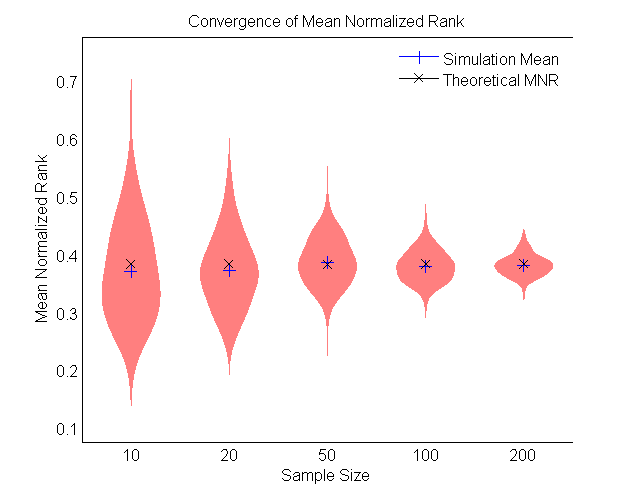
\includegraphics[width=4in]{simumnr_violin}
\end{center}
\caption{Simulation results}
\end{figure*}

\subsection{Simulation Experiment: Comparing MNR and I2C2}
\noindent In this subsection, we use simulated data to demonstrate the utility of MNR. In addition, comparison is made between MNR and another reliability measure I2C2. I2C2 is another reliability measure introduced in paper (**). Under additive noise assumption, I2C2 is defined to be one minus the ratio of within subject variance over total variance. That is given $O_{ij}=X_i+Z_{ij}$,
 
\[ I2C2=1-\frac{\text{Trace}(\text{Cov}(Z_{ij}))}{\text{Trace}(\text{Cov}(O_{ij}))} \]

In practice, $\text{Cov}(Z_{ij})$ and $\text{Cov}(O_{ij})$ need to be estimated from data. Compared to I2C2, MNR has a few advantages. First, MNR is a more generalized and non-parametric measure of reliability. MNR can be easily extended to non-Euclidean metric and still be able to interpreted as a probability. Due to the fact that MNR rely on fewer assumptions and only estimate the probability, it turns out that relative standard error of MNR estimate is usually less than I2C2. Furthermore, non-additive noise and non-continuous data cannot be properly handled by I2C2. Even in continuous and additive noise setting, I2C2 is only determined by first two moments of data and is not sensitive to higher moments or correlations between noises.\\
\\
In the coming experiment, we consider four data generation scheme. We assume there are only two subjects under study, and $50$ observations in $\mathbb{R}^2$ are generated for each subject. Then we compute ICC of the first dimension, ICC of the second dimension, I2C2 and MNR. For each data generation scheme, $100$ repetitions are done. The figure 2 shows the result.\\
\\
\textbf{Scheme 1:} The noise is additive independent multivariate normal distribution. That is $O_{ij}=X_i+Z_{ij}$, where $X_1=[1,1]$, $X_2=[1,-1]$ and $Z_{ij}\sim\text{MVN}(0,(\begin{matrix} 1 & 0 \\ 0 & 2\end{matrix}))$. \\
\textbf{Scheme 2:} The data is generately essentially the same as scheme 1, but rotated $\frac{\pi}{4}$. That is $O_{ij}=X_i+Z_{ij}$, where $X_1=[\sqrt{2},0]$, $X_2=[0,-\sqrt{2}]$, $Z_{ij}\sim\text{MVN}(0,(\begin{matrix} 1.5 & 0.5 \\ 0.5 & 1.5\end{matrix}))$. \\
\textbf{Scheme 3:} The noise is still additive but generated from Laplacian distribution. That is $O_{ij}=X_i+Z_{ij}$, where $X_1=[1,1]$, $X_2=[1,-1]$. The first dimension of $Z_{ij}$ is generated from $\text{Laplace}(0,\frac{1}{\sqrt{2}})$, and the second dimension is generated from $\text{Laplace}(0,1)$. The parameters are chosen to make sure two subject conditional distributions has the same mean and covariance matrix as in scheme 1. \\
\textbf{Scheme 4:} The noise is multiplicative generated from log-normal distribution. That is $O_{ij}=X_i*Z_{ij}$, where $X_1=[1,1]$, $X_2=[1,-1]$  and $Z_{ij}\sim\text{LN}([\ln{2},\ln{3}],(\begin{matrix} \ln{2} & 0 \\ 0 & \ln{3}\end{matrix}))$. The parameters are chosen to make sure two subject conditional distributions has the same mean and covariance matrix as in scheme 1. \\
\begin{figure*}[t!]
\begin{center}
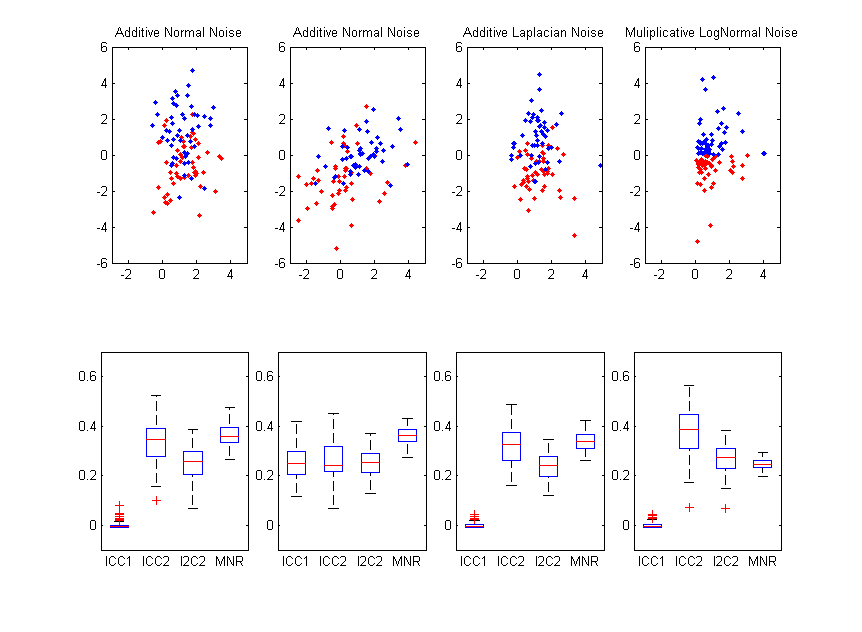
\includegraphics[width=5in]{Simu1}
\end{center}
\caption{Simulation results}
\end{figure*}

\noindent In figure 1, the scatter plots at the top are observations from two subjects, and the box plots at the bottom are the corresponding reliability measures. First, it is not surprising that one dimensional reliability measure ICC does not capture reliability of higher dimensional data. Comaring scheme 1 and scheme 2, we expect that simple rotation does not affect reliability; however, ICCs of two dimensions change substantially. Second, we can see I2C2 does not fully reflect the reliability of data. In all four cases, I2C2 are roughly the same due to the fact we fix the first and second moments of data. However, we can see from the scatter plots that observations of scheme 3 is slightly more separated than observations of scheme 1, and observations of scheme 4 is mostly separated. At last, I2C2 clearly has larger estimation variance than MNR. This is partly due to the fact that I2C2 have more parameters to estimate. In order to compute I2C2, we must first estimate diagonal terms of two covariance matrices which leads to large variance in I2C2 estimate.   \\
\\
In this simple setting, we can quantify the degree of separation between two subjects by using Bayes error. Two subjects can be treated as two classes, and the Bayes errors of four schemes are $0.2395$, $0.2395$, $0.1839$ and $0$ respectively. It can be seen that MNR respects this ordering and reflects the degree of separation between subjects.   If we are interested in predicting a phenotype, our intuition is that the error rate will more likely to be small, when there is more separation between subjects. We conclude here that MNR is a better reliability measure.


\subsection{Simulation Experiment: Maximizing Reliability}
\noindent In this experiment, we demonstrate reliability can be used to select parameter in data preprocessing. As in the last section, we consider only 2 subjects, each with s observations in $\mathbb{R}^2$. Again, we consider additve noise setting. The means of two subjects are $X_1=[1,0]$ and $X_2=[-1,0]$ respectively. For the noise, we consider two cases. The first case is $Z_{ij}\sim\text{MVN}([0,0],(\begin{matrix} 4 & 0 \\ 0 & 1\end{matrix}))$ and the second case is $Z_{ij}\sim\text{MVN}([0,0],(\begin{matrix} 1 & 0 \\ 0 & 4\end{matrix}))$. \\
\\
Now, assuming we want to linearly project the observations into 1 dimensional space. To achieve this, we sample possible lines to project uniformly from sphere, and compute reliability of projection. Then, we choose the projection which has maximum MNR. Also, PCA is performed for comparison. Because of the way that data is generated, we see the optimal linear projection should be projecting observations onto x-axis, and Bayes error is the same before and after this projection. The figure 3 shows the result. From the figure, we see both MNR PCA give the optimal projection in the first case. However, in the second case only MNR gives the optimal projection. In this case, the second dimension has larger variance than the first dimension; therefore, PCA choose y-axis to project to.

\begin{figure*}[t!]
\begin{center}
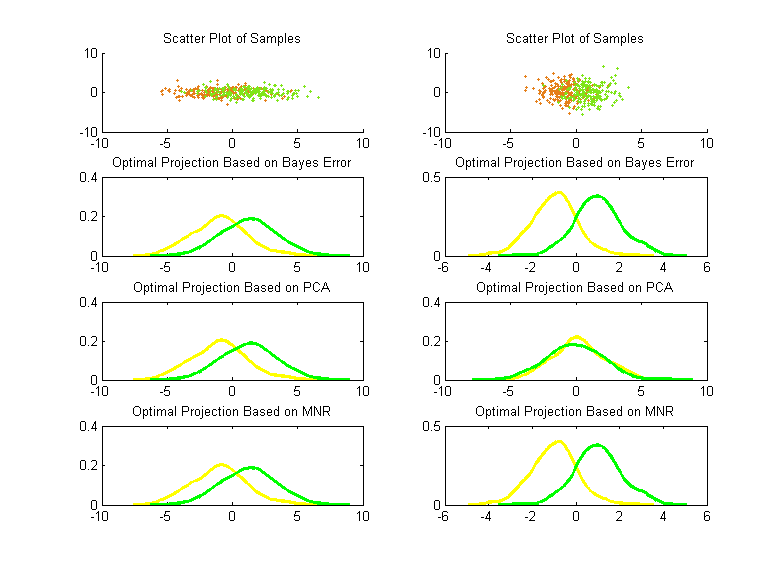
\includegraphics[width=4in]{parameter_selection_2sub}
\end{center}
\caption{Simulation results}
\end{figure*}


\section{Real Data Experiment}
\subsection{Human Connectome Data: NKI}
The first real data set analyzed is a human connectome data set NKI. There are $176$ subjects in the data set and each subject's brain is scanned twice ($n=176$, $s=2$). The original time series data is parcellized and the brain is divided into $131$ and $165$ regions. We first compute a correlation matrix which record correlations between different regions of the brain. The correlation matrix is then thresholded by $t$. Specifically, there is an edge between two regions if and only if the absolute correlation between two regions are greater than $t$. In this way, we construct a graph from each brain scan.\\ 
\\
Despite brain scans, demographic information including age and gender of subjects is also collected. The inference task is to predict age and gender of a subject based on the graph derived from his or her brain scan. K-Nearest Neighbor rule is applied to predict both age and gender. In this experiment, we are interested in how to correctly select the threshold $t$ and how the threshold affects inference results. Figure 4 and 5 summarize the results.\\



\noindent From figure 4 and 5, we can see the processed data is most reliable when the threshold $t$ is around $0.16$. Meanwhile, mean squared error of age prediction and classification error of gender prediction are also close to their minimums. Gender and age are two uncorrelated variables in the data set. Therefore, this experiment demonstrates that processed data of maximum reliability is optimal for two independent inference tasks. 

\subsection{Human Connectome Data: HCP}
HCP is another human connectome data set we analyze. In the data set, 476 subjects are each scanned 4 times. Scans are then parcellized into 25, 50, 100, 200 and 300 regions. Again we compute the correlation matrix and threshold it to construct a graph for each brain scan. Age and gender are then predicted based on the constructed graph.\\


\noindent Figure 6-10 show similar results. The most reliable processed data has smallest classification error. However, mean square error of age prediction seems to just fluctuate randomly. This may due to the fact that age prediction is a much harder task and the K-NN is not good enough to capture the change of differentiability of processed data.\\
\\
A natural question to ask next is that among these 7 connectome data sets which one is most reliable. The question can be answered by comparing MNR. For each data set, we first choose the threshold $t$ which maximizes reliability and then compare the corresponding MNR across data set. A standard error estimate is also calculated by assuming normalized ranks are independent. The assumption leads to underestimate the standard error due to mild positive correlations between normalized ranks. To test whether two data sets are of same reliability, we can construct to confidence intervals of MNR and check whether they overlap or not. \\
\\
Table 1 below summarizes the results. Two NKI data sets are remarkably more reliable compared to 5 HCP data sets. Reliability of NKI131 tends to be better than reliability of NKI165, but the difference is not statistical significant. Among 5 HCP data sets, HCP100 tends to be the most reliable one. By looking at HCP data sets alone, we discover another interesting fact that reliability demonstrates some kinds of bias-variance tradeoff. When the brain is partitioned into very few regions, the data set is not reliable possibly due to large bias. When the brain is partitioned into a large number of regions, the data set is also not reliable due to large variance. 

\begin{table}

\begin{center}
  \begin{tabular}{| p{2.5 cm} | p{2.5 cm} | p{2.5 cm} |}
    \hline
    Data Set & Mean Rank & S.E. \\ \hline
    NKI131 & 0.0151 & 0.0034 \\ \hline
    NKI165 & 0.0215 & 0.0044 \\ \hline
    HCP25 & 0.1393 & 0.0030 \\ \hline
    HCP50 & 0.1077 & 0.0029 \\ \hline
    HCP100 & 0.0753 & 0.0024 \\ \hline
    HCP200 & 0.0843 & 0.0026 \\ \hline
    HCP300 & 0.0944 & 0.0027 \\ \hline
%    \hline
  \end{tabular}
  \caption{Reliability Comparison}
\end{center}
\end{table}




\section{Conclusion}
In the sections above, we demonstrate that maximizing reliability helps improving prediction accuracy. Our work provides guidance and direction to scientists on data preprocessing. Particularly, when facing decisions which are hard to make in data preprocessing, scientists should consider preprocessing method which maximizes reliability of processed data.\\
\\
The current work can be extended in both theoretical and practical directions. From theoretical aspect, we only show Bayes error rate varies with reliability. It is also interesting to see the classification error of a specific classifier varies with reliability. Secondly, assumptions of theoretical analysis should be relaxed. Assumptions include additive noise, independence between noise and true values, and Euclidean distance maybe relaxed to better model real data. Thirdly, we only analyze the relationship between classification and reliability. More inference tasks should be considered. These inference tasks can be but not limit to hypothesis testing, regression and clustering. Their relationship to reliability should be investigated.\\
\\ 
From the aspect of practice, the whole data preprocessing procedure should be studied. In the experiments above, we focus on only one step of the data preprocessing. We may investigate reliability of data preprocessing step as a whole or even starting at data collection step. Secondly, more data experiments should be done in different setting to prove utility of reliability in data preprocessing. Data of more complicated form or with non-Euclidean distance can be investigated in a similar manner. The points mentioned in this and last paragraph can all extend our current work and improve its applicability. Nevertheless, our primary purpose is to demonstrate the relationship between reliability and predictability.





\appendices
\section{Proof of Lemmas}
%\subsubsection*{Proof for Lemma 1}
\begin{proof}[Proof of Lemma 1]
By definition of $R$,
\[E(R)= \frac{\sum\limits_{i=1}^{n} \sum\limits_{j=1}^{s}  \sum\limits_{k=1,k\neq j}^{s} E(R_{ijk})}{ns(s-1)}\]
The expectation of $R_{ijk}$ can be simplified,
\begin{eqnarray*}  
& &E(R_{ijk}) \\
&=&\frac{\sum\limits_{p=1,p\neq i}^{n} \sum\limits_{q=1}^{s} E(I\{\|O_{ij}-O_{pq}\| < \|O_{ij}-O_{ik}\| \}) }{(n-1)s} \\
&=&\frac{\sum\limits_{p=1,p\neq i}^{n} \sum\limits_{q=1}^{s} P(\|O_{ij}-O_{pq}\| < \|O_{ij}-O_{ik}\| ) }{(n-1)s} \\
&=&P(\|O_{ij}-O_{pq}\| < \|O_{ij}-O_{ik}\|) \text{ for any $p\neq i$}
\end{eqnarray*}
The last equality is due to the fact that $O$s have the same distribution. Notice the symmetry of $R_{ijk}$ in $i$, $j$ and $k$ we have,
\[E(R)=E(R_{ijk})=P(\|O_{ij}-O_{pq}\| < \|O_{ij}-O_{ik}\|)\]
\end{proof}

\begin{proof}[Proof of Lemma 2]
By definition of $R$,
\begin{eqnarray*}  
R &=&\frac{\sum\limits_{i,j,k,k\neq j} R_{ijk}}{ns(s-1)}\\
&=& \frac{\sum\limits_{i,j,k,k \neq j,p,p\neq i,q} I_{ijkpq}}{ns(s-1)(n-1)s}\\
\end{eqnarray*}
Here, $I_{ijkpq}:=I\{\|O_{ij}-O_{pq}\| < \|O_{ij}-O_{ik}\| \}$. We show in the previous lemma that $E(R)=P(\|O_{ij}-O_{pq}\| < \|O_{ij}-O_{ik}\|)$. To demonstrate that $R$ converges to its epxectation in probability, it is suffice to show that $\text{Var}(R) \rightarrow 0$. Since then, by Chebyshev's inequality,
\[P(|R-E(R)| \geq \epsilon) \leq \frac{\text{Var}(R)}{\epsilon^2} \rightarrow 0\]
If we expand the variance of $R$, 
\[\text{Var}(R)= \frac{\sum\limits_{i,j,k,p,q} \sum\limits_{i',j',k',p',q'} \text{Cov}(I_{ijkpq},I_{i'j'k'p'q'})}{(ns(s-1)(n-1)s)^2} \]
There are $(ns(s-1)(n-1)s)^2$ terms in the sum at the nominator; however, some of them are actually 0. $I_{ijkpq}$ is a function of $O_{ij}$, $O_{ik}$ and $O_{pq}$; therefore, is independent of any observations of subjects other than $i$ and $p$. This implies $I_{ijkpq}$ is independent of $I_{i'j'k'p'q'}$ as long as $\{i,p\} \cap \{i',p'\} = \emptyset$. As a consqeunce, there are $(4n-6)(s(s-1)s)2=ns(s-1)(n-1)s-(n-2)s(s-1)(n-3)s$ combinations of $i'j'k'p'q'$ such that covariance between $I_{ijkpq}$ and $I_{i'j'k'p'q'}$ maybe non-zero. Furthermore, the covariance must be less $\frac{1}{4}$ due to the fact that they are indicator random variables. Therefore, we have 
\begin{eqnarray*} 
\text{Var}(R)&=& \frac{\sum\limits_{i,j,k,p,q} \sum\limits_{i',j',k',p',q'} \text{Cov}(I_{ijkpq},I_{i'j'k'p'q'})}{(ns(s-1)(n-1)s)^2} \\
&\leq& \frac{\sum\limits_{i,j,k,p,q}  (4n-6)(s(s-1)s)}{4(ns(s-1)(n-1)s)^2} \\
&=& \frac{ (ns(s-1)(n-1)s)(4n-6)(s(s-1)s)}{4(ns(s-1)(n-1)s)^2} \\
&=& \frac{(4n-6)}{4n(n-1)} \\
&\leq& \frac{1}{n}  \\
&\rightarrow& 0 \text{ , as $n\rightarrow \infty$} 
\end{eqnarray*}
As discussed above, this concludes the proof for the lemma.
\end{proof}

\begin{proof}[Proof of Lemma 3]
By Lemma 1, we only need to bound $P(\|O_{ij}-O_{ik}\| < \|O_{ij}-O_{pq}\|)$. Under additive noise setting,
\begin{eqnarray*}
& &P(\|O_{ij}-O_{ik}\| < \|O_{ij}-O_{pq}\|) \\
&=&P(\|Z_{ij}-Z_{ik}\| < \|X_{i}+Z_{ij}-X_{p}-Z_{pq}\|) \\
&\geq&P(\|Z_{ij}-Z_{ik}\| < \|X_{i}-X_{p}\| - \|Z_{ij}-Z_{pq}\|) \\
&=& P(\|Z_{ij}-Z_{ik}\|+\|Z_{ij}-Z_{pq}\|< \|X_{i}-X_{p}\|) \\
&\geq& P(\|Z_{ij}-Z_{ik}\|^2+\|Z_{ij}-Z_{pq}\|^2< \|X_{i}-X_{p}\|^2) \\
\end{eqnarray*}
To bound the probability above, we bound the two terms on different sides of equation separately. We start with the term at the left side and compute its expectation.
 \begin{eqnarray*}
 & &E(\|Z_{ij}-Z_{ik}\|^2+\|Z_{ij}-Z_{pq}\|^2) \\
 &=&2 E(\|Z_{ij}-Z_{ik}\|^2) \\
 &=&2 E(Z_{ij}^T Z_{ij}+Z_{ik}^T Z_{ik} +2Z_{ij}^T Z_{ik}) \\
 &=&4\sigma_1^2
 \end{eqnarray*}
 We then use Markov's Inequality to this term, 
 \[P(\|Z_{ij}-Z_{ik}\|^2+\|Z_{ij}-Z_{pq}\|^2 < k\sigma_1^2) \geq 1-\frac{4}{k} \]
 Similarly, we compute the expectation of second term.
  \begin{eqnarray*}
  & &E(\|X_{i}-X_{p}\|^2) \\
  &=&E(X_{i}^T X_{i}+X_{p}^T X_{p}+2X_{i}^T X_{p}) \\
  &=&2\sigma_2^2 \\
  &=&2\lambda^2\sigma_1^2
  \end{eqnarray*}
Then, we apply Paley-Zygmund Inequality,
\[P(\|X_i-X_p\|^2 > k\sigma_1^2 ) \geq c(1-\frac{k}{2\lambda^2})^2 \]
Understand the fact that $X$s and $Z$s are independent, we can combine the two inequalities and get a bound on $P(\|O_{ij}-O_{ik}\| < \|O_{ij}-O_{pq}\|)$.
\begin{eqnarray*}
& &P(\|O_{ij}-O_{ik}\| < \|O_{ij}-O_{pq}\|) \\
&\geq& P(\|Z_{ij}-Z_{ik}\|^2+\|Z_{ij}-Z_{pq}\|^2< \|X_{i}-X_{p}\|^2) \\
&\geq& P(\|Z_{ij}-Z_{ik}\|^2+\|Z_{ij}-Z_{pq}\|^2<k\sigma_1^2) \\
& & \times P(\|X_i-X_p\|^2 > k\sigma_1^2 ) \\
&\geq& c(1-\frac{k}{2\lambda^2})^2(1-\frac{4}{k}) \\
&=&c(1-\frac{\sqrt{2}}{\lambda})^3
\end{eqnarray*}
The last equality is the result by setting $k=2\sqrt{2}\lambda$. This leads to the final result on the expectation of mean normalized rank.
\begin{eqnarray*}
E(R)&=&1-P(\|O_{ij}-O_{ik}\| < \|O_{ij}-O_{pq}\|) \\
&\leq& 1-c(1-\frac{\sqrt{2}}{\lambda})^3
\end{eqnarray*}
We can also solve for and lower bound $\lambda$.
\[\lambda \geq \frac{2^{\frac{1}{4}}}{1-(\frac{1-E(R)}{c})^{\frac{1}{3}}} \]
\end{proof}


\begin{proof}[Proof of Lemma 4]
To compute Mahalanobis distance, we first compute weighted covariance matrix.
\begin{eqnarray*}
\text{Var}(O|Y=i) &=& \text{Var}(X|Y=i)+\text{Var}(Z|Y=i) \\
&=& \Sigma_i+\frac{1}{\lambda^2}\Sigma
\end{eqnarray*}
Therefore, the weighted covariance matrix of $O$s
\begin{eqnarray*}
\Sigma_\lambda&=&\pi_0\text{Var}(O|Y=0)+\pi_1\text{Var}(O|Y=1) \\
&=&\pi_0\Sigma_0+\pi_1\Sigma_1+\frac{1}{\lambda^2}\Sigma
\end{eqnarray*}
Then, apply Devijver and Kittler's result,
\[L_\lambda \leq \frac{2\pi_0\pi_1}{1+\pi_0\pi_1(\mu_0-\mu_1)^T\Sigma_\lambda^{-1}(\mu_0-\mu_1)}\]
\end{proof}

% you can choose not to have a title for an appendix
% if you want by leaving the argument blank


% use section* for acknowledgement
\ifCLASSOPTIONcompsoc
  % The Computer Society usually uses the plural form
  \section*{Acknowledgments}
\else
  % regular IEEE prefers the singular form
  \section*{Acknowledgment}
\fi


The authors would like to thank...


% Can use something like this to put references on a page
% by themselves when using endfloat and the captionsoff option.
\ifCLASSOPTIONcaptionsoff
  \newpage
\fi



% trigger a \newpage just before the given reference
% number - used to balance the columns on the last page
% adjust value as needed - may need to be readjusted if
% the document is modified later
%\IEEEtriggeratref{8}
% The "triggered" command can be changed if desired:
%\IEEEtriggercmd{\enlargethispage{-5in}}

% references section

% can use a bibliography generated by BibTeX as a .bbl file
% BibTeX documentation can be easily obtained at:
% http://www.ctan.org/tex-archive/biblio/bibtex/contrib/doc/
% The IEEEtran BibTeX style support page is at:
% http://www.michaelshell.org/tex/ieeetran/bibtex/
%\bibliographystyle{IEEEtran}
% argument is your BibTeX string definitions and bibliography database(s)
%\bibliography{IEEEabrv,../bib/paper}
%
% <OR> manually copy in the resultant .bbl file
% set second argument of \begin to the number of references
% (used to reserve space for the reference number labels box)
%\begin{thebibliography}{1}

%\bibitem{IEEEhowto:kopka}
%H.~Kopka and P.~W. Daly, \emph{A Guide to \LaTeX}, 3rd~ed.\hskip 1em plus
%  0.5em minus 0.4em\relax Harlow, England: Addison-Wesley, 1999.

%\end{thebibliography}

% biography section
% 
% If you have an EPS/PDF photo (graphicx package needed) extra braces are
% needed around the contents of the optional argument to biography to prevent
% the LaTeX parser from getting confused when it sees the complicated
% \includegraphics command within an optional argument. (You could create
% your own custom macro containing the \includegraphics command to make things
% simpler here.)
%\begin{biography}[{\includegraphics[width=1in,height=1.25in,clip,keepaspectratio]{mshell}}]{Michael Shell}
% or if you just want to reserve a space for a photo:

%\begin{IEEEbiography}{Michael Shell}
%Biography text here.
%\end{IEEEbiography}

% if you will not have a photo at all:
%\begin{IEEEbiographynophoto}{John Doe}
%Biography text here.
%\end{IEEEbiographynophoto}

% insert where needed to balance the two columns on the last page with
% biographies
%\newpage

%\begin{IEEEbiographynophoto}{Jane Doe}
%Biography text here.
%\end{IEEEbiographynophoto}

% You can push biographies down or up by placing
% a \vfill before or after them. The appropriate
% use of \vfill depends on what kind of text is
% on the last page and whether or not the columns
% are being equalized.

%\vfill

% Can be used to pull up biographies so that the bottom of the last one
% is flush with the other column.
%\enlargethispage{-5in}



% that's all folks
\end{document}


